% $Id$
%

%%---------------------------------------------------------------
%%---------------------------------------------------------------
\section{Prácticas: Introducción a Django}

%%---------------------------------------------------------------
\begin{frame}
\frametitle{Enfoques comunes de desarrollo web}

\begin{itemize}
\item Frameworks de desarrollo web
  \begin{itemize}
  \item PHP, JavaEE, Python+HttpServer...
  \end{itemize}
\item Entornos de desarrollo web completos
  \begin{itemize}
  \item Django (Python), \url{http://djangoproject.org}
  \item Ruby on Rails (Ruby), \url{http://rubyonrails.org/}
  \item CakePHP (PHP), \url{http://cakephp.org/}
  \item Grails (Groovy, sovre JVM), \url{http://grails.org/}
  \item RIFE (Java), \url{http://rifers.org/}
  \end{itemize}
\item Plataformas extensibles
  \begin{itemize}
  \item CMS: Joomla, Drupal...
  \item Portal: Plone/Zope, Liferay Portal...
  \item Plataformas de propósito específico: Moodle, Wordpress...
  \end{itemize}
\end{itemize}

\end{frame}


%%---------------------------------------------------------------
\begin{frame}
\frametitle{¿Qué es Django?}

\begin{itemize}
\item Entorno integrado de desarrollo de aplicaciones web
\item Herramientas para gestionar la aplicación
\item Framework (armazón) para presentación de la aplicación
\item Acceso a base de datos (correspondencia objeto-relacional)
\item Seguridad (XSS, SQL Injection, ...)
\item Componentes listos para usar (gestión de usuarios, sesiones, interfaz administración,...)
\item \emph{Caché}, internacionalización, plantillas, etc.
\end{itemize}

\begin{flushright}
\url{http://docs.djangoproject.com/}
\end{flushright}
\end{frame}

%%---------------------------------------------------------------
\begin{frame}
\frametitle{Otras plataformas Python similares a Django}

Flask: \url{https://flask.palletsprojects.com/}
\begin{itemize}
\item Aproximación minimalista, centrada en la simplicidad
\item Con extensiones, funcionalidad similar a Django
\end{itemize}

\vspace{0.5cm}

FastAPI: \url{https://fastapi.tiangolo.com/}:

\begin{itemize}
\item Especialmente orientada a APIs HTTP
\item Se apoya en el tipado de Python
\end{itemize}

\end{frame}

%%---------------------------------------------------------------
\begin{frame}
\frametitle{Django: conceptos principales}

\begin{itemize}
\item Objetivo principal: desarrollo muy rápido
  \begin{itemize}
  \item Entorno integrado y completo
  \item Cambios en caliente
  \item Descripciones de error muy descriptivas
  \item Convenciones preferible a configuración
  \item Evitar duplicación a toda costa (DRY, don't repeat yourself)
  \end{itemize}
\item Desarrollo dirigido por el modelo
  \begin{itemize}
  \item Se comienza por el diseño del modelo de datos
  \end{itemize}
\end{itemize}

\end{frame}


%%---------------------------------------------------------------
\begin{frame}[fragile]
\frametitle{Preparativos}

\begin{itemize}
\item Usaremos una versión de Django 5.0.3, instalándola vía pip3.
\item Disponible para Linux, *BSD, Windows, MacOS, etc.
\item Creación de entorno virtual:

\begin{verbatim}
% python3 -m venv django-venv    
\end{verbatim}

\item Activación del entorno virtual:

\begin{verbatim}
% source django-venv/bin/activate
\end{verbatim}

\item Instalación de Django en el entorno virtual:

\begin{verbatim}
% pip3 install django==5.0.3
\end{verbatim}

\item Comprobación (debe responder 5.0.3):
\begin{verbatim}
% django-admin --version
\end{verbatim}
\end{itemize}


\end{frame}


%%---------------------------------------------------------------
%\begin{frame}[fragile]
%\frametitle{Preparativos (y II)}

%\begin{itemize}
%\item Preparación de entorno (necesario si no se ha instalado en path ``habituales'', como p.ej. en el laboratorio):
%\begin{verbatim}
%export DJANGO=/home/al-..-../..../.../Django-1.7.5/
%   # Camino al directorio con fuentes descomprimidas
%export PATH=$DJANGO/django/bin:$PATH
%export PYTHONPATH=$DJANGO:$PYTHONPATH
%\end{verbatim}
%\item Incluir los tres exports anteriores en el fichero ~/.bashrc para que se ejecuten con cada nuevo terminal.
%\item Abrir un nuevo terminal y comprobar que funciona (ver paso anterior).
%\end{itemize}
%
%\end{frame}

%%---------------------------------------------------------------
\begin{frame}[fragile]
\frametitle{Armazón para proyecto y aplicación}

\begin{itemize}
\item Creación (primero proyecto, luego aplicación)
\begin{verbatim}
$ cd dir-practica
$ django-admin startproject myproject
$ cd myproject
$ python3 manage.py startapp myfirstapp
\end{verbatim}
\item Más opciones de manage.py
\begin{verbatim}
$ python3 manage.py --help
\end{verbatim}
\item Ejecución de la aplicación (\url{http://localhost:8000})
\begin{verbatim}
$ python3 manage.py runserver
\end{verbatim}
%\item Creación de las bases de datos:
%\begin{verbatim}
%$ python3 manage.py migrate
%\end{verbatim}

\end{itemize}

\end{frame}

%%---------------------------------------------------------------
\begin{frame}[fragile]
\frametitle{Ficheros creados para un proyecto}

\begin{itemize}
  \item Raíz:
  \begin{itemize}
    \item \verb|manage.py|: herramienta para gestionar el proyecto
  \end{itemize}
  \item Proyecto : \verb|myproject/|:
  \begin{itemize}
    \item \verb|__init__.py|: fichero vacío, directorio debe ser considerado un paquete Python
    \item \verb|settings.py|: configuración del proyecto
    \item \verb|urls.py|: URLs del proyecto
    \item \verb|wsgi.py|: fichero para servir Django mediante WSGI (p.ej. con Apache)
    \item \verb|asgi.py|: fichero para servir Django mediante ASGI (servidor asíncrono)
  \end{itemize}
\end{itemize}

\end{frame}

%%---------------------------------------------------------------
\begin{frame}[fragile]
\frametitle{Ficheros creados para una aplicación}


\begin{itemize}
\item Raíz:
  \begin{itemize}
  \item Aplicación (\verb|myfirstapp/|):
    \begin{itemize}
      \item \verb|__init__.py|: fichero vacío, directorio debe ser considerado un paquete Python
      \item \verb|views.py|: vistas (código invocado para cada recurso)
       \item \verb|models.py|: definición de las clases del modelo de datos
       \item \verb|admin.py|: registro de los modelos que se pueden gestionar vía web
       \item \verb|apps.py|: configuración de la app
       \item \verb|tests.py|: fichero para la implementación de tests
       \item \verb|migrations/|: versiones (y \emph{migraciones}) de los modelos
    \end{itemize}
  \end{itemize}
\end{itemize}

Generalmente, también se crea un \verb|urls.py|, con las URLs de la aplicación.

\end{frame}

%%---------------------------------------------------------------
\begin{frame}[fragile]
\frametitle{Fichero settings.py}

\begin{itemize}
\item Fichero de configuración, en Python
\item Configuración de la base de datos (usaremos SQLite3)
\begin{verbatim}
DATABASES = {
    'default': {
        'ENGINE': 'django.db.backends.sqlite3',
        'NAME': os.path.join(BASE_DIR, 'db.sqlite3'),
    }
}
\end{verbatim}
\item Aplicaciones instaladas
\begin{verbatim}
INSTALLED_APPS = [
    ...,
]
\end{verbatim}
\item Otros: zona horaria, codificación, directorio de plantillas...
\end{itemize}

\end{frame}


%%---------------------------------------------------------------
\begin{frame}[fragile]
\frametitle{Declaración de URLs (proyecto)}

\begin{itemize}
\item En el fichero urls.py (del proyecto): \verb|myproject/urls.py|
\item Ejemplo:

\begin{verbatim}
from django.contrib import admin
from django.urls import include, path

urlpatterns = [
    path('myfirstapp/', include('myfirstapp.urls')),
    path('admin/', admin.site.urls),
]
\end{verbatim}


\item \verb|include()| permite añadir otros \verb|urls.py| de aplicaciones

\end{itemize}

%\begin{flushright}
%{\small
%\url{http://es.wikipedia.org/wiki/Expresi\%C3\%B3n_regular}
%\url{https://docs.djangoproject.com/en/dev/topics/http/urls/}
%}
%\end{flushright}


\end{frame}



%%---------------------------------------------------------------
\begin{frame}[fragile]
\frametitle{Declaración de URLs (aplicación)}

En el fichero urls.py (de la aplicación): \verb|myfirstapp/urls.py|

\begin{verbatim}
from django.urls import path
from . import views

urlpatterns = [
    path('', views.index, name='index'),
    path('hello', views.say_hello, name='hello'),
    path('bye/<name>', views.say_bye_to, name='bye'),
    path('number/<int:number>', views.say_number, name='number')
]
\end{verbatim}

\end{frame}

%%---------------------------------------------------------------
%% \begin{frame}[fragile]
%% \frametitle{Declaración de URLs: La función \emph{url}}

%% \verb|url(regex, view, kwargs=None, name=None, prefix='')|

%% \begin{itemize}
%%   \item \verb|regex|: expresión regular.
%%   \begin{itemize}
%%     \item No tiene en cuenta si la petición es GET o POST, o el dominio
%%     \item Se ejecuta la primera que se encuentra (i.e., el orden importa)
%%   \end{itemize} 
%%   \item \verb|view|: función \emph{vista} a la que se llama, pasándole:
%%   \begin{itemize}
%%     \item Como primer parámetro un objeto HttpRequest con la petición
%%     \item Otros posibles parámetros como argumentos
%%   \end{itemize} 
%%   \item \verb|kwargs|: diccionario con parámetros adicionales a la vista.
%%   \item \verb|name|: nombre de la URL (muy útil para plantillas).
%%   \item \verb|prefix|: deprecated a partir de Django 1.8
%% \end{itemize}

%% \end{frame}

%---------------------------------------------------------------
\begin{frame}[fragile]
\frametitle{Declaración de URLs: La función path}

\verb|path(route, view, kwargs=None, name=None)|

\begin{itemize}
 \item \verb|route|: patrón de la URL.
 \begin{itemize}
   \item No tiene en cuenta si la petición es GET o POST, o el dominio
   \item Se ejecuta la primera que se encuentra (i.e., el orden importa)
 \end{itemize} 
 \item \verb|view|: función \emph{vista} a la que se llama, pasándole:
 \begin{itemize}
   \item Como primer parámetro un objeto HttpRequest con la petición
   \item Otros posibles parámetros como argumentos
 \end{itemize} 
 \item \verb|kwargs|: diccionario con parámetros adicionales a la vista.
 \item \verb|name|: nombre de la URL (muy útil para plantillas).
\end{itemize}

\end{frame}

%%---------------------------------------------------------------
\begin{frame}[fragile]
\frametitle{Views}

\begin{itemize}
\item Código invocado para una URL o conjunto de URLs
\item Debe ser un método (o un objeto)
\item Los métodos se definen en el fichero \verb|myfirstapp/views.py|
\item Ejemplo:
\begin{verbatim}
from django.http import HttpResponse

def index(request):
     return HttpResponse('<h1>Welcome to my App!</h1>')
def say_hello(request):
     return HttpResponse('Hello!')
def say_bye_to(request, name):
     return HttpResponse('Bye %s'%name)
def say_number(request, number=0):
     return HttpResponse('Number: %s'%number)
\end{verbatim}
\end{itemize}
\end{frame}


%%---------------------------------------------------------------
\begin{frame}[fragile]
\frametitle{Gestión de datos persistentes}

\begin{itemize}
\item Django hace corresponder un objeto Python con cada tabla
\item Cada aplicación tiene su models.py
  \begin{itemize}
  \item Una clase por cada entidad (tabla) del modelo
  \item Un campo por cada dato (columna) de la entidad
  \item \_\_str\_\_() da una representación del objeto (p.ej., un campo)
  \item Ejemplo:
\begin{verbatim}
from django.db import models

class MyFirstAppData(models.Model):
    name = models.CharField(max_length=200)
    birthday = models.DateTimeField()
    
    def __str__(self):
        return self.name
\end{verbatim}
  \end{itemize}
\item Creación de tablas
\begin{verbatim}
$ python manage.py makemigrations
$ python manage.py migrate
\end{verbatim}
\end{itemize}

\end{frame}


%%---------------------------------------------------------------
\begin{frame}
\frametitle{Definición del modelo}

\begin{itemize}
\item Tipos de campos:
  \begin{itemize}
  \item CharField(maxlength)
  \item TextField()
  \item IntegerField()
  \item DateField()
  \item BooleanField()
  \end{itemize}
\item Relaciones:
  \begin{itemize}
  \item ForeignKey(othermodel)
  \item ManyToManyField('self', symmetrical=False)
  \end{itemize}
\end{itemize}
\begin{flushright}
\url{http://docs.djangoproject.com/en/dev/ref/models/fields/}
\end{flushright}

\end{frame}

%%---------------------------------------------------------------
\begin{frame}
\frametitle{Migraciones de datos}

Cuando se modifica el modelo, puede existir una inconsistencia con los datos en la base de datos. ¡Peligro: se pueden perder datos!

\begin{itemize}
  \item El proceso de migraciones se encarga de la propagación de modificaciones en el modelo (p.ej., añadir/borrar un campo)
  \item \texttt{makemigrations}: crea nuevas migraciones, basándose en los cambios a los modelos.
  \item \texttt{migrate}: aplica la migración, además de listar el estado.
%  \item \texttt{sqlmigrate}: muestra las instrucciones SQL de la migración.
  \item Los archivos para las migraciones se encuentran en el directorio \texttt{migrations} de las aplicaciones. Se crean automáticamente con \texttt{makemigrations}, aunque (luego) se pueden modificar a mano.
  \item \texttt{createsuperuser}: crea un usuario superusuario para poder entrar en el interfaz de admin admin
\end{itemize}

\end{frame}


%%---------------------------------------------------------------
\begin{frame}[fragile]
\frametitle{Admin site}

Versión simple:

\begin{itemize}
\item INSTALLED\_APPS (en settings.py) ha de incluir:
  \begin{itemize}
  \item django.contrib.admin
  \item django.contrib.sessions (dependencia del anterior)
  \item ...y lo necesario para usuarios
  \end{itemize}
\item Hay que crear las tablas pertinentes (manage.py migrate)
\item Enganche en urls.py
\begin{verbatim}
from django.contrib import admin
urlpatterns = [
    url('^admin/', include(admin.site.urls)),
]    
\end{verbatim}
\end{itemize}
\end{frame}

%%---------------------------------------------------------------
\begin{frame}[fragile]
\frametitle{Admin site (2)}

Ahora, proporcionemos interfaz para nuestra tabla Pages:

\begin{itemize}
\item Crea en el directorio de la aplicación Django de gestión de contenidos el fichero admin.py
\item Registra en él los modelos a manejar:
\begin{verbatim}
from django.contrib import admin
from .models import Pages

admin.site.register(Pages)
\end{verbatim}
\item Prueba que ahora puedes manejar esta tabla desde el sitio de administración
\end{itemize}
\end{frame}



%%---------------------------------------------------------------
\begin{frame}
\frametitle{Consultas a la base de datos}

\begin{itemize}
\item Métodos para realizar consultas a la base de datos
\item Acceso a entradas de la base de datos mediante el objeto 'objects' \\
  (ej. MyFirstAppData.objects)
\item Métodos:
\begin{itemize}
\item MyFirstAppData.save()
\item MyFirstAppData.objects.all()
\item MyFirstAppData.objects.filter(campo=valor)
\item MyFirstAppData.objects.get(campo=valor) \\
  Excepción si no lo encuentra
\end{itemize}
\end{itemize}

\end{frame}


%%---------------------------------------------------------------

\begin{frame}[fragile]
\frametitle{Modelos: relación muchos a uno (ForeignKey)}

\begin{verbatim}
class Manufacturer(models.Model):
    # ...
class Car(models.Model):
    manufacturer = models.ForeignKey(Manufacturer)
    # ...
\end{verbatim}


\begin{verbatim}
# Creating
m = Manufacturer(name='Seat')
c = Car(name='Toledo')
m.save(); c.save()
# Relationship
c.manufacturer = m
# Obtaining
c.manufacturer
c.manufacturer.id
\end{verbatim}

\end{frame}


%%---------------------------------------------------------------
\begin{frame}[fragile]
\frametitle{Acceso al modelo desde las vistas}

\begin{itemize}
\item Las vistas pueden usarse para leer y modificar al modelo
\begin{verbatim}
from django.http import HttpResponse,HttpResponseNotFound
from content.models import Pages

def show_content(request, resource):
    try:
        record = Pages.objects.get(name=resource)
        return HttpResponse(record.page)
    except Pages.DoesNotExist:
        return HttpResponseNotFound(
            'Page not found: /%s.' % resource
            )
\end{verbatim}
\end{itemize}
\end{frame}

%%---------------------------------------------------------------
\begin{frame}[fragile]
\frametitle{Seguridad}

\begin{itemize}
  \item Django viene con alguna protección de seguridad por defecto
  \item Por ejemplo, CSRF: \emph{Cross-site request forgery} o falsificación de petición en sitios cruzados
  \item Si el POST/PUT no incluye un csrf\_token creado con anterioridad por el servidor, da un error de seguridad
  \item Se evita con el @csrf\_exempt para un método concreto en views.py
\end{itemize}

\begin{verbatim}
from django.views.decorators.csrf import csrf_exempt
@csrf_exempt
def vista(request):
    if request.method == "POST":
        return HttpResponse("Has enviado " + request.body)
\end{verbatim}

\end{frame}


%%---------------------------------------------------------------
\begin{frame}
\frametitle{Usuarios}

\begin{itemize}
\item INSTALLED\_APPS (en settings.py) ha de incluir:
  \begin{itemize}
  \item django.contrib.auth
  \item django.contrib.contenttypes
  \end{itemize}
\item Hay que crear las tablas pertinentes (manage.py migrate)
\end{itemize}
\end{frame}


%%---------------------------------------------------------------
\begin{frame}[fragile]
\frametitle{Acceso a información de usuario y logout}

\begin{itemize}
\item Accedemos a información del objeto User, que tenemos en HTTPRequest
\item En views.py:
\begin{verbatim}
def show_content(request, resource):
  if request.user.is_authenticated:
    logged = 'Logged in as ' + request.user.username
  else:
    logged = 'Not logged in.'
\end{verbatim}
\item Para logout, utilizamos función. En views.py:
\begin{verbatim}
from django.contrib.auth import logout

def logout_view(request):
    logout(request)
    return redirect("/")
\end{verbatim}
\end{itemize}
\end{frame}


%%---------------------------------------------------------------
\begin{frame}[fragile]
\frametitle{Login}

\begin{itemize}
\item Utilizamos view predefinida (entiende GET y POST)
\item En urls.py:
\begin{verbatim}
from django.contrib.auth.views import login
urlpatterns = [
    url(r'^login', login),
]
\end{verbatim}
\item Necesita una plantilla registration/login.html:
  \begin{itemize}
  \item En settings.py:
\begin{verbatim}
TEMPLATES = [
  {
    'DIRS': ['templates'], # para todas las apps del proyecto
  },
]
\end{verbatim}
  \item Creación de templates/registration/login.html
  \end{itemize}
\end{itemize}

\begin{flushright}
Info detallada: ``User authentication in Django''
\end{flushright}
\end{frame}

%%---------------------------------------------------------------
\begin{frame}[fragile]
\frametitle{templates/registration/login.html}

\begin{verbatim}
<html><body>
<form method="post" action="/login">

<table>
  <tr><td>Username</td>
      <td>{{ form.username }}</td></tr>
  <tr><td>Password</td>
      <td>{{ form.password }}</td></tr>
</table>
<input type="submit" value="login" />
</form>
</body></html>
\end{verbatim}
\end{frame}




%%---------------------------------------------------------------
\begin{frame}
\frametitle{Model View Controller (el tradicional)}

\begin{center}
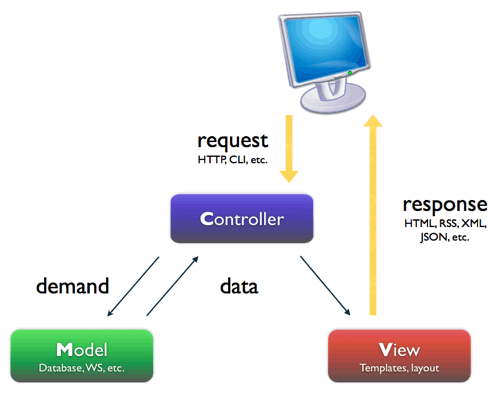
\includegraphics[width=8cm]{figs/mvc.png}
\end{center}

\begin{flushright}
{\footnotesize
Fuente: \url{http://djangoexamples.blogspot.com.es/2013/05/about-django-mvc.html}
}
\end{flushright}
\end{frame}

%%---------------------------------------------------------------
\begin{frame}
\frametitle{Model View Template (el de Django)}

\begin{center}
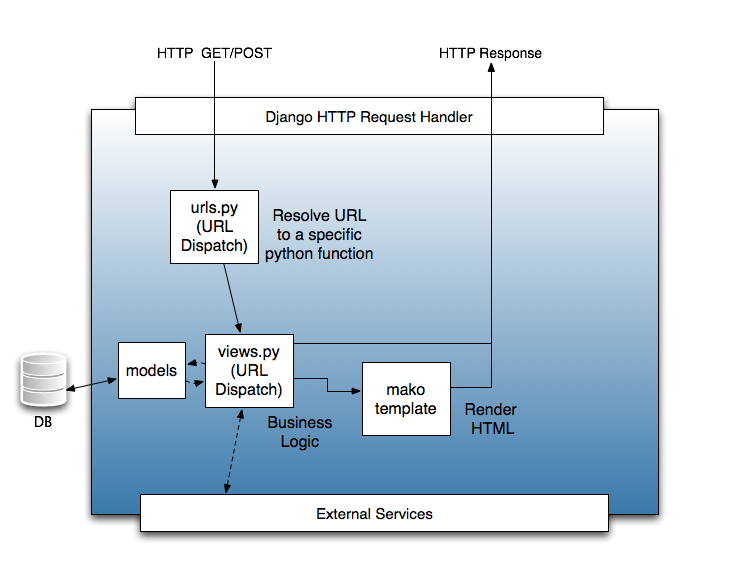
\includegraphics[width=8cm]{figs/mvc-mtv-django}
\end{center}

\begin{flushright}
{\footnotesize
Fuente: \url{http://archive.cloudera.com/cdh4/cdh/4/hue/sdk/sdk.html}
}
\end{flushright}
\end{frame}


%%---------------------------------------------------------------
\begin{frame}
\frametitle{Plantillas (templates)}

\begin{itemize}
\item Ficheros de texto que pueden generar cualquier formato basado en texto (HTML, XML, CSV, etc.)
\item Contienen:
  \begin{itemize}
  \item Texto (que queda igual)
  \item Variables (reemplazadas por su valor cuando se evalúan)
  \item Filtros (modifican variables cuando se evalúan)
  \item Etiquetas (controlan la lógica de la evaluación de la plantilla)
  \item Comentarios \{\# Comentario \#\}
  \end{itemize}
\item Pueden extender (heredar de) otras plantillas
\item Se colocan en los directorios de plantillas (TEMPLATE\_DIRS en settings.py) 
\end{itemize}
\end{frame}

%%---------------------------------------------------------------
\begin{frame}[fragile]
\frametitle{Plantillas: variables y filtros}

\begin{itemize}
\item Variables: 
\begin{verbatim}
    {{ variable }}
\end{verbatim}
\item Filtros:
\begin{verbatim}
    {{ variable|filtro|otrofiltro }}
\end{verbatim}
\item Filtro con argumentos:
\begin{verbatim}
    {{ variable|filtro:30 }}
\end{verbatim}
\item Ejemplos de filtros:
\begin{verbatim}
    {{ value|default:"nothing" }}
    {{ value|length }}
    {{ text|striptags }}
    {{ text|truncatewords:30 }}
    {{ text|escape|linebreaks }}
    {{ list|join:", " }}.
\end{verbatim}
\end{itemize}
\end{frame}

%%---------------------------------------------------------------
\begin{frame}[fragile]
\frametitle{Ejemplo de plantilla}

\begin{verbatim}
<html>
  <body>
    <div id="title">
      {{ title }}
    </div>

    <div id="content">
      {{ content }}
    </div>
  </body>
</html>
\end{verbatim}

\end{frame}


%%---------------------------------------------------------------
\begin{frame}[fragile]
\frametitle{Plantillas: uso en vistas}

Directorios con plantillas:
\begin{itemize}
  \item directorio templates en directorio de la app
  \item lista DIRS en variable TEMPLATES en settings.py
\end{itemize}
 
\begin{verbatim}
from django.shortcuts import render

def view (request):
    ...
    return(render(request, 'template.html',
                  {'title': title,
                   'content': content}))
\end{verbatim}
\end{frame}

%%---------------------------------------------------------------
\begin{frame}[fragile]
\frametitle{Plantillas: uso en vistas (2)}

 
\begin{verbatim}
from django.template import loader

def view (request):
    ...
    template = loader.get_template('template.html')
    html = template.render({'title': title,
                            'content': content},
                           request)
    return(HttpResponse(html, status=status))
\end{verbatim}
\end{frame}

%%---------------------------------------------------------------
\begin{frame}[fragile]
\frametitle{Plantillas (avanzado): etiquetas}

\begin{itemize}
\item ifequal, ifnotequal
\begin{verbatim}

    ...


    ...

\end{verbatim}
\item block: Indica bloques a redefinir en plantillas que hereden
\item extends: Hereda de plantilla madre (sólo hace falta redefinir
 \emph{blocks} que se quieren modificar)
\end{itemize}
\end{frame}


%%---------------------------------------------------------------
\begin{frame}[fragile]
\frametitle{Herencia en Plantillas: Ej. plantilla ``madre'' (base.html)}

\begin{verbatim}
<body>
  <div id="sidebar">
  
    <ul>
     <li><a href="/">Home</a></li>
     <li><a href="/blog/">Blog</a></li>
    </ul>
  
  </div>

  <div id="content">
     
  </div>
</body>
</html>
\end{verbatim}

\end{frame}


%%---------------------------------------------------------------
\begin{frame}[fragile]
\frametitle{Ejemplo de plantilla que hereda (plantilla.html)}

\begin{verbatim}


  {{ title }}



  <h1>{{ title }}</h1>
  
  <h2>
    <a href="{{ story.get_absolute_url }}">
      {{ story.headline|upper }}
    </a>
  </h2>
  <p>{{ story.tease|truncatewords:"100" }}</p>
  

\end{verbatim}

\end{frame}


%%---------------------------------------------------------------

\begin{frame}[fragile]
\frametitle{Modelos: relación muchos a muchos (ManyToManyField)}

\begin{verbatim}
class Topping(models.Model):
    name = models.CharField(max_length=32)
class Pizza(models.Model):
    name = models.CharField(max_length=32)
    toppings = models.ManyToManyField(Topping)
\end{verbatim}

\end{frame}

%%---------------------------------------------------------------

\begin{frame}[fragile]
\frametitle{Modelos: relación muchos a muchos (ManyToManyField) (2)}

\begin{verbatim}
pb = Pizza(name='Barbecue')
pq = Pizza(name='4 Cheese')
b = Topping(name='Barbecue sauce')
m = Topping(name='Mozzarela')
pb.save(); pp.save(); b.save(); m.save()
pb.toppings.add(b, m)
pq.toppings.add(m)
pq.toppings.create(name='Rochefort')
m.pizza_set.all()
pb.toppings.all()
Pizza.objects.filter(toppings__name='Mozzarela')
\end{verbatim}

\end{frame}



%%---------------------------------------------------------------

\begin{frame}[fragile]
\frametitle{Ficheros estáticos con Django}

\begin{itemize}
\item Los ficheros estáticos no se deberían servir con Django...
\item (lo hace mucho mejor un servidor web como Apache o Cherokee)
\item ...pero se pueden servir
\item django.views.static.serve()

\begin{verbatim}
from django.views.static import serve

urlpatterns = [
  url(r'^css/(.*)$', serve, {'document_root': 'sfiles'}),
]
\end{verbatim}

\end{itemize}

(donde sfiles es un subdirectorio que cuelga del proyecto)

\end{frame}



%%---------------------------------------------------------------
\begin{frame}[fragile]
\frametitle{Plantillas: uso en urls.py}

\begin{verbatim}
from django.conf.urls.defaults import *
from django.views.generic.simple import direct_to_template

urlpatterns = [
    url(r'^about$', direct_to_template, {
        'template': 'about.html'
    }),
]
\end{verbatim}
\end{frame}



%%---------------------------------------------------------------
\begin{frame}[fragile]
\frametitle{Otras acciones de gestión del proyecto}

\begin{itemize}
\item Ejecución en el contexto de Python con acceso al código de la aplicación
\begin{verbatim}
% python manage.py shell
\end{verbatim}
\item Validacion de modelos de datos
\begin{verbatim}
% python manage.py validate
\end{verbatim}
\item Exportación de datos de la base de datos
\begin{verbatim}
% python manage.py dumpdata
\end{verbatim}
\item Importación de datos en la base de datos
\begin{verbatim}
% python manage.py loaddata
\end{verbatim}
\end{itemize}

\end{frame}


%%---------------------------------------------------------------
\begin{frame}[fragile]
\frametitle{Plantillas (avanzado): etiquetas}

\begin{itemize}
\item for
\begin{verbatim}

    <li>{{ athlete.name }}</li>

\end{verbatim}
\item if
\begin{verbatim}

    Number of athletes: {{ athlete_list|length }}

    No athletes.

\end{verbatim}

\end{itemize}
\end{frame}


%%---------------------------------------------------------------
\begin{frame}[fragile]
\frametitle{La shell de Django}

Acceso a la API de los objetos de nuestro proyecto

\begin{verbatim}
% python manage.py shell
>>> from myproject.myfirstapp.models import MyFirstAppData
>>> MyFirstAppData.objects.all()
[]
>>> p = MyFirstAppData(name="Jesus",
                       birthday="2009-05-05")
>>> p.save()
>>> p.id
1
>>> MyFirstAppData.objects.filter(name="Jesus")
...
>>> MyFirstAppData.objects.get(pk=1).name
u'Jesus'
\end{verbatim}

\end{frame}



%%---------------------------------------------------------------

\begin{frame}[fragile]
\frametitle{Generador de canales}

\begin{itemize}
\item Django viene con módulos para generar canales RSS y Atom
\item View de alto nivel que genera el canal (feed):

\begin{verbatim}
(r'^feeds/(?P<url>.*)/$', 'django.contrib.syndication.views.feed',
   {'feed_dict': feeds}),
\end{verbatim}

\item Hay que proporcionar un diccionario con la correspondencia canal a objeto Feed:

\begin{verbatim}
feeds = {
    'latest': LatestEntries,
    'categories': LatestEntriesByCategory,
}
\end{verbatim}
\end{itemize}

\end{frame}

%%---------------------------------------------------------------

\begin{frame}[fragile]
\frametitle{Generador de canales: objetos Feed}

\begin{itemize}
\item Representan los datos de un canal:

\begin{verbatim}
from django.contrib.syndication.feeds import Feed
from content.models import Pages

class LatestEntries(Feed):
    title = "My CMS contents"
    link = "/feed/"
    description = "Contents of my CMS."

    def items(self):
        return Pages.objects.order_by('-pub_date')[:5]
\end{verbatim}

\item También hay que definir plantillas (templates) para $<$title$>$ y $<$description$>$ de cada item del canal RSS
\end{itemize}

\end{frame}

%%---------------------------------------------------------------

\begin{frame}[fragile]
\frametitle{Tests}

\begin{itemize}
\item Pruebas de comportamiento del programa
\item Pruebas ``internas'' (vía llamadas directas) \\
  Usando \verb|django.test| (que extiende \verb|unittest|)
\item Pruebas ``externas'' (via API HTTP) \\
  Usando el ``Django test client''
\item Permite probar también plantillas, formularios, modelos...
\item Normalmente, en fichero \verb|tests.py|
\end{itemize}

{\small
\begin{verbatim}
% ./manage.py test
Creating test database for alias 'default'...
System check identified no issues (0 silenced).
........
----------------------------------------------------------------------
Ran 8 tests in 0.022s

OK
Destroying test database for alias 'default'...
\end{verbatim}
}

\begin{flushright}
\url{https://docs.djangoproject.com/en/3.1/topics/testing/}
\end{flushright}

\end{frame}

%%---------------------------------------------------------------

\begin{frame}[fragile]
\frametitle{Tests (pruebas internas)}

{\small
\begin{verbatim}
from django.test import TestCase
from . import views

class TestViews(TestCase):

    def setUp(self):
        """Ejecutado antes de los tests"""
        ...

    def test_simple(self):
        """Test de la función aux"""
        result = views.aux(...)
        self.assertEqual(result, expected)
\end{verbatim}
}

\end{frame}

%%---------------------------------------------------------------

\begin{frame}[fragile]
\frametitle{Tests (pruebas API HTTP)}

{\small
\begin{verbatim}
from django.test import SimpleTestCase
from . import views

class TestHTTP(SimpleTestCase):
    """Tests of HTTP API"""

    def setUp(self):
        """Ejecutado antes de los tests"""
        ...

    def test_get_ok(self):
        response = self.client.get('/')
        self.assertEqual(response.status_code, 200)
        self.assertEqual(response.resolver_match.func, views.main)
        self.assertInHTML("<h1>Title</h1>",
                response.content.decode(encoding='UTF-8'))
\end{verbatim}
}

\end{frame}


%%---------------------------------------------------------------

\begin{frame}[fragile]
\frametitle{Internacionalización}

\begin{itemize}
\item Cadenas de traducción en código Python

\begin{verbatim}
from django.utils.translation import ugettext as _

def my_view(request):
    output = _("Welcome to my site.")
    return HttpResponse(output)

def my_view(request, m, d):
    output = _('Today is %(month)s, %(day)s.') % 
       {'month': m, 'day': d}
    return HttpResponse(output)
\end{verbatim}

\end{itemize}

\end{frame}

%%---------------------------------------------------------------

\begin{frame}[fragile]
\frametitle{Internacionalización (2)}

\begin{itemize}
\item Cadenas de traducción en plantillas

\begin{verbatim}
<title></title>


This string will have {{ value }} inside.

\end{verbatim}

\end{itemize}

\end{frame}

%%---------------------------------------------------------------

\begin{frame}[fragile]
\frametitle{Internacionalización (3)}

\begin{itemize}
\item Traducciones en los lenguajes requeridos

\begin{verbatim}
django-admin.py makemessages -l es
\end{verbatim}

\item Activar el soporte para locale en Django

\begin{verbatim}
MIDDLEWARE_CLASSES = (
 'django.contrib.sessions.middleware.SessionMiddleware',
 'django.middleware.locale.LocaleMiddleware',
 'django.middleware.common.CommonMiddleware',
)
\end{verbatim}

\end{itemize}

\end{frame}

%%---------------------------------------------------------------
\begin{frame}
\frametitle{Referencias}

\begin{itemize}
\item Documentación de Django \\
  \url{http://docs.djangoproject.com/en/dev}
\item Libro de Django \\
  \url{http://www.djangobook.com}
\item Documentación de Python \\
  \url{http://www.python.org/doc/}
\item Tutorial sobre Django (e introducción a Django) \\
\url{http://docs.djangoproject.com/en/dev/intro}
\end{itemize}

\end{frame}


